\section{Introduction}

On-policy distillation (OPD)~\citep{agarwal2024policy,gu2024minillm} transfers reasoning and generation ability from a strong teacher to a smaller student. Unlike offline distillation \citep{kim-rush-2016-sequence} or supervised fine-tuning, it trains the student on self-generated trajectories with token-level teacher supervision, which reduces exposure bias over long sequences. OPD is now a standard step in Large Language Model (LLM) post-training at frontier labs, including Thinking Machines \citep{lu2025onpolicydistillation}, GLM \citep{zeng2026glm}, and DeepSeek \citep{xu2026deepseek}.

Standard OPD \citep{agarwal2024policy} needs the teacher's full distribution at every generated token,
which is prohibitively costly for modern LLMs whose vocabularies can reach 250K tokens,
so the payload grows with vocabulary size per token and with rollout length per sequence. Practical training systems therefore expose a sparse teacher interface that, at each step, returns only the teacher's Top-$k$ tokens with their probabilities, along with the probability of the sampled token \citep{zhang2026ema,huang2026tail}. We refer to OPD trained through such an interface as \textbf{sparse OPD}. The difficulty is that the omitted tail is never observed: objectives defined directly on the Top-$k$ support, whether by truncation or renormalization \citep{zhu2026many} or by aggregating the omitted mass into a ghost token \citep{anshumann-etal-2025-sparse,huang2026tail}, are surrogates of the full-vocabulary reverse Kullback-Leibler (rKL) objective and carry a systematic gradient bias (Fig.~\ref{fig:estimator-anatomy}(b)).

Bias can be traded for variance: rather than shrinking the objective to the observed support, a second family of methods retains the full-vocabulary rKL objective and estimates its gradient from the sparse payload, remaining \textbf{unbiased but noisy}. However, existing estimators fail to fully exploit this payload. At one extreme, sampled-token OPD \citep{gu2024minillm,lu2025onpolicydistillation} queries only the rollout token's score, suffering from severe gradient variance due to single-sample Monte Carlo estimation (Fig.~\ref{fig:estimator-anatomy}(b)). At the other, methods with Top-$k$ access underutilize it: scalar-baseline variants such as vOPD \citep{oh2026kl} reduce the head to a detached baseline rather than evaluating its token-wise gradient analytically (Tab.~\ref{tab:mechanism}), while hybrid schemes such as \citet{zhang2026ema}, which we refer to as Head-Exact Tail-Sampled (HETS), evaluate the head exactly but treat the tail correction as entirely unknown despite knowing its aggregate mass. Consequently, each tail hit must compensate for the entire omitted mass, injecting large gradient spikes; even at 98.4\% head coverage, a 30K-token reasoning trace contains 460--470 such spikes, thousands per optimizer step (Sec.~\ref{sec:train_dynamics}).
Practitioners are thus left choosing between a biased objective and an unstable gradient, which causes sampled-token OPD and HETS to peak early and degrade later in training (Sec.~\ref{sec:math-opd}).

\begin{figure}[t]
\centering
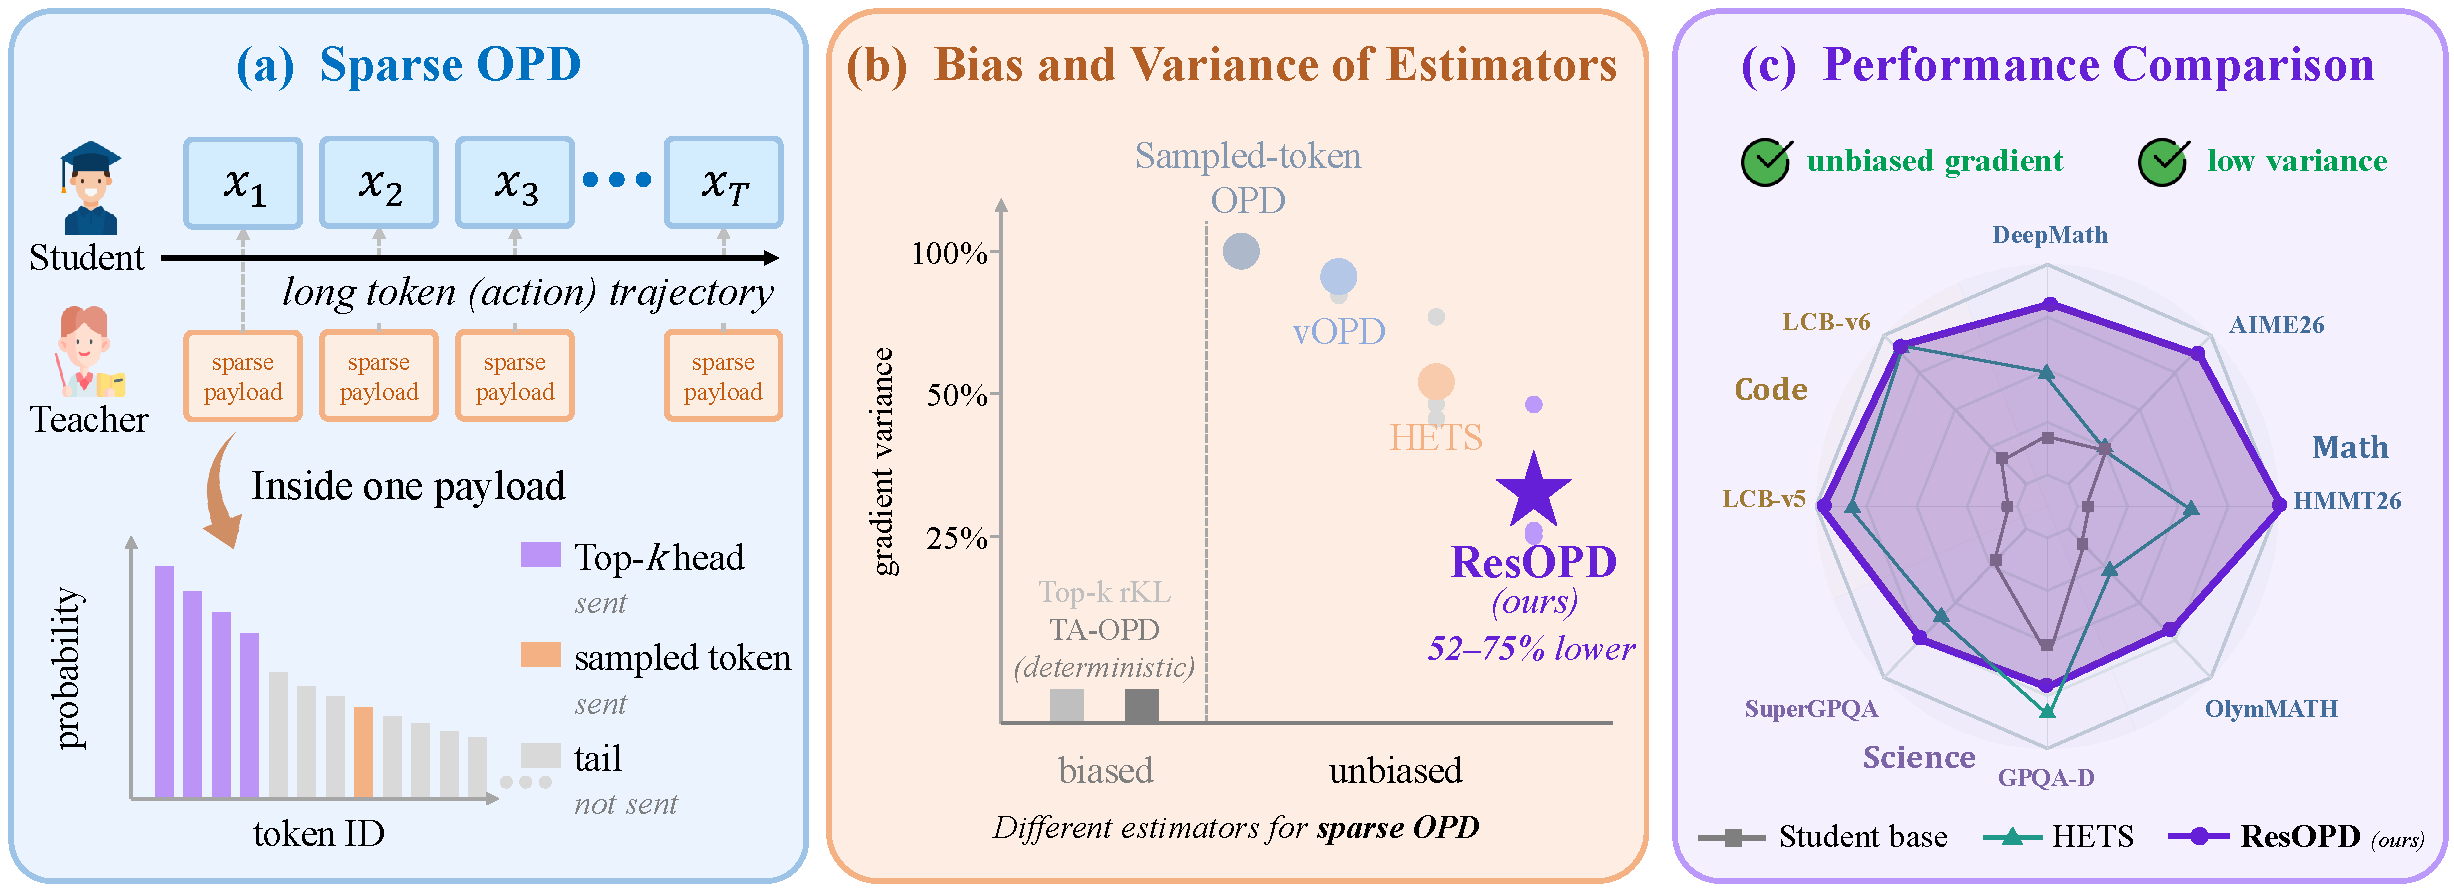
\includegraphics[width=1.0\textwidth]{figs/teaser_v21.pdf}
\caption{(a) Sparse OPD: the teacher model only sends the Top-$k$ head probabilities and the sampled token score, leaving the tail distribution unobserved. (b) Bias vs.\ variance trade-off: while deterministic Top-$k$ surrogates suffer from systematic gradient bias, ResOPD provides an unbiased gradient estimator and substantially reduces gradient variance. (c) Downstream evaluation: the radar chart shows benchmark scores across mathematics, coding, and science; while the relative ranking varies by task, ResOPD achieves the best overall performance.}
\label{fig:estimator-anatomy}
\vspace{-4mm}
\end{figure}

To resolve this trade-off, we analyze sparse OPD at the level of the gradient estimator. We first show that any estimator evaluating the head exactly, adding a prefix-dependent control vector weighted by the student's tail mass, and correcting on tail hits is unbiased for the full-vocabulary rKL gradient, with HETS as the special case of a zero control (Sec.~\ref{subsec:cfr}). Our covariance-trace decomposition reveals that variance splits into an invariant within-tail sampling term and a between-event term proportional to the control's distance from the true tail mean. This explains HETS's gradient spikes: its zero control pays for the full tail mean on every hit, whereas any control that better predicts this mean strictly reduces variance. Crucially, the residual masses outside the head define a coarse pseudo-token \citep{anshumann-etal-2025-sparse,huang2026tail} whose analytical gradient serves as a computable tail-mean predictor. Building on this, we propose \textit{\textbf{O}n-\textbf{P}olicy \textbf{D}istillation with Tail \textbf{Res}idualization} (\method{}): at every step it computes the exact gradient of the $(k+1)$-way coarse distribution, adding only a small residual correction on tail hits (Fig.~\ref{fig:framework}(a)). The resulting estimator is provably unbiased while retaining the same sparse teacher payload.

We evaluate \method{} in two settings. In exact frozen-prefix audits that enumerate every next-token action, \method{} lowers the gradient covariance trace by 52--75\% relative to sampled-token OPD under Top-$4$ feedback, below both HETS and a payload-matched vOPD baseline (Tab.~\ref{tab:mechanism}). In end-to-end distillation from Qwen3.5-27B to Qwen3.5-4B, it attains the best average score among the evaluated sparse OPD baselines on four mathematical reasoning benchmarks, 4.40 points above HETS under the same payload (Tab.~\ref{tab:math-terminal}),
and its average advantage over HETS consistently holds across every tested support size $k\in\{1,4,16,32\}$, with small margins (Tab.~\ref{tab:topk-breakdown}).

Our contributions are as follows:
(1) \textbf{Bias and variance analysis of sparse OPD.} We show that truncated, renormalized, and stopped-coefficient Top-$k$ rKL objectives are all biased surrogates of the full-vocabulary objective, and we derive a covariance-trace decomposition that separates within-tail sampling variance from between-event variance. This yields the exact condition under which a coarse tail control lowers variance relative to HETS, and a two-control family in which HETS, \method{}, and the concurrent SC-TA \citep{huang2026tail} appear as special cases.
(2) \textbf{\method{} estimator.} We propose an estimator that splits the full-vocabulary rKL gradient into an exact $(k+1)$-way coarse term, computed at every step from the Top-$k$ payload and the residual tail masses, and a within-tail residual correction applied only when the rollout token lands in the tail. The estimator is unbiased under on-policy sampling and requires no additional teacher queries or forward passes.
(3) \textbf{Empirical validation.} Using exact frozen-prefix gradient audits and end-to-end distillation settings, we show that \method{} reduces gradient covariance, lowers online residual moments during training, and improves downstream accuracy over the evaluated sparse OPD baselines.
